\documentclass[11pt,a4paper]{article}

\usepackage[margin=2.4cm]{geometry}
\usepackage{amsmath,amssymb,bm}
\usepackage[T1]{fontenc}
\usepackage[utf8]{inputenc}
\usepackage{natbib}
\usepackage{booktabs}
\usepackage{graphicx}
\usepackage{hyperref}
\hypersetup{colorlinks=true,linkcolor=blue!50!black,citecolor=blue!50!black,urlcolor=blue!50!black}
\usepackage{xcolor}

\bibliographystyle{plainnat}
\setcitestyle{authoryear,round}
\sloppy

\newcommand{\pMpc}{\,{\rm pMpc}}
\newcommand{\Msun}{\,M_\odot}

\title{\bf Neutral vs.\ Fully Ionized Medium: Which Takes Longer\\ to Cool an Injected Electron, and Why?\\[2mm]
\large Response record for \texttt{electron\_energy\_loss\_neutral\_medium.py}, following Master Rule 2}
\author{Prepared for L.\ Carvalho}
\date{5 September 2026}

\begin{document}
\maketitle

\begin{abstract}
\noindent
This note repeats the electron energy-loss calculation of
\texttt{electron\_energy\_loss\_response.tex}, but for the electron traveling through
\texttt{igm\_losses.py}'s own, \emph{unmodified}, default medium --- the mostly neutral high-$z$
intergalactic medium ($x_e=n_e/n_H=10^{-4}$) that module was originally built for --- rather than the
fully ionized bubble interior. Both media are run in a single execution of
\texttt{electron\_energy\_loss\_neutral\_medium.py} (same folder, producing
\texttt{electron\_energy\_loss\_neutral\_medium.png} and \texttt{electron\_medium\_comparison.png}) for a
like-for-like comparison. The result is unambiguous and fully explained by the dominant loss mechanism in
each medium: \textbf{the neutral medium takes longer to cool at every injection energy tested},
by a factor that falls from $\sim21\times$ at $10^3$~eV to a floor of $\sim1.4\times$ above $10^7$~eV.
\end{abstract}

\tableofcontents

%=====================================================================
\section{Assumptions}
\label{sec:assumptions}

\begin{enumerate}
\item Identical source, injection redshift ($z_{\rm inject}=z_{\rm form}=20$), injection point ($r=0$), and
      $K_{\rm ini}$ grid ($10^3$--$10^{12}$~eV) as \texttt{electron\_energy\_loss\_response.tex}; only the
      medium differs.
\item \textbf{Neutral medium:} \texttt{igm\_losses.py}'s own, completely unmodified
      \texttt{loss\_rates()}/\texttt{n\_HI(z)}, i.e.\ $x_e=10^{-4}$ (mostly neutral), $n_{\rm HI}(z)$ its
      built-in cosmic mean hydrogen density normalization (already cross-checked against this folder's own
      Planck 2018 $n_H(z)$ to $2.3\%$ in \texttt{electron\_energy\_loss\_response.tex}). No adaptation was
      needed for this task --- this \emph{is} the module's intended, as-built use case.
\item \textbf{Fully ionized medium:} the identical bubble-interior physics of
      \texttt{electron\_energy\_loss\_in\_bubble.py} ($n_e=n_H(z)$, residual
      $x_{\rm HI}(r,z)$ from \citealt{Cen2000} for the collisional terms), reproduced self-contained in the
      same script execution so both media are compared under identical numerical conditions (solver,
      tolerances, cosmology) in one run.
\item Both trajectories are integrated from injection to thermalization ($K=1.5\,k_BT_{\rm CMB}(z)$) or
      $z=5$, whichever comes first; ``time to cool'' means time to thermalization.
\end{enumerate}

%=====================================================================
\section{Derivation}
\label{sec:derivation}

The only difference between the two runs is the pair of densities entering the Coulomb term (free
electrons) and the collisional excitation/ionization terms (neutral hydrogen atoms) of
\texttt{igm\_losses.py}'s eq.~(loss\_rates), reused verbatim in both cases:
\begin{center}
\begin{tabular}{@{}lcc@{}}
\toprule
 & neutral medium (\texttt{igm\_losses.py} default) & fully ionized bubble \\
\midrule
$n_e$ (Coulomb) & $10^{-4}\,n_H(z)$ & $n_H(z)$ \\
$n_{\rm HI}$ (excitation/ionization) & $\approx n_H(z)$ & $x_{\rm HI}(r,z)\,n_H(z) \ll n_H(z)$ \\
\bottomrule
\end{tabular}
\end{center}
Synchrotron, inverse Compton, adiabatic expansion and bremsstrahlung are identical in both cases (none
depend on the free/bound partition of the hydrogen).

%=====================================================================
\section{Verification / cross-check}
\label{sec:verification}

\begin{enumerate}
\item \textbf{Dominant mechanism at injection ($z=20$), by medium:}
\begin{center}
\begin{tabular}{@{}lccc@{}}
\toprule
$K_{\rm ini}$ (eV) & dominant, neutral & dominant, ionized & rate ratio (ionized/neutral) \\
\midrule
$10^3$ & ionization & Coulomb & $7.11$ \\
$10^4$ & ionization & Coulomb & $4.48$ \\
$10^5$ & Compton    & Coulomb & $2.25$ \\
$\ge10^6$ & Compton & Compton & $1.00$ \\
\bottomrule
\end{tabular}
\end{center}
      At low energy the two media lose energy through \emph{different} channels entirely: collisional
      ionization of neutral hydrogen (neutral medium) vs.\ Coulomb scattering off free electrons (ionized
      medium). Despite comparable target densities ($n_{\rm HI}\approx n_e\approx n_H(z)$ in their
      respective regimes), the instantaneous Coulomb loss rate is $4$--$7\times$ \emph{faster} than the
      collisional-ionization rate at the same $K$ and $z$: Coulomb scattering off free electrons is a
      long-range ($1/r$ potential) process with a logarithmically enhanced cross section (the Gould 1972
      Coulomb logarithm), whereas collisional excitation/ionization of a bound electron is a
      finite-range, threshold process with a smaller effective cross section per encounter. At
      $K\ge10^6$~eV both media are Compton-dominated (rate ratio exactly $1.00$), since inverse-Compton
      scattering off the CMB does not depend on the hydrogen ionization state at all.
\item \textbf{Thermalization-time cross-check:} the fully-ionized-bubble times reproduced here
      ($0.0015$--$11.90$~Myr across the $K_{\rm ini}$ grid) match
      \texttt{electron\_energy\_loss\_response.tex}'s Table~1 and printed output exactly (same physics,
      re-run in this script for a single, consistent execution) --- confirming no drift between the two
      scripts.
\item \textbf{Full thermalization-time comparison:}
\begin{center}
\begin{tabular}{@{}lccc@{}}
\toprule
$K_{\rm ini}$ (eV) & $t_{\rm therm}$, neutral (Myr) & $t_{\rm therm}$, ionized (Myr) & ratio \\
\midrule
$10^3$  & $0.031$  & $0.0015$ & $21.4$ \\
$10^4$  & $0.239$  & $0.043$  & $5.59$ \\
$10^5$  & $3.23$   & $1.04$   & $3.10$ \\
$10^6$  & $11.95$  & $7.12$   & $1.68$ \\
$10^7$  & $16.24$  & $11.18$  & $1.45$ \\
$10^8$--$10^{12}$ & $16.89$--$16.96$ & $11.83$--$11.90$ & $1.425$--$1.428$ \\
\bottomrule
\end{tabular}
\end{center}
      The ratio is monotonically decreasing with $K_{\rm ini}$ and asymptotes to $\approx1.425$, never
      reaching $1$ even though the dominant mechanism is identical (Compton) at high $K_{\rm ini}$: every
      electron, however energetic at injection, must eventually cascade down through the low-energy regime
      where the two media genuinely differ, and that fixed extra delay ($\approx5.06$~Myr in absolute
      terms at high $K_{\rm ini}$: $16.96-11.90$) becomes a progressively smaller \emph{fractional}
      correction as $K_{\rm ini}$ grows, but never vanishes.
\end{enumerate}

%=====================================================================
\section{Final result}
\label{sec:final}

\textbf{The neutral hydrogen medium takes longer to cool an injected electron than the fully ionized bubble
interior, at every injection energy from $10^3$ to $10^{12}$~eV.} The effect is largest at low energy
($21\times$ longer at $1$~keV) and shrinks to a floor of $\approx1.4\times$ above $\sim10^7$~eV. The reason
is the identity of the dominant loss channel at each energy:
\begin{itemize}
\item \emph{Low energy ($\lesssim10^5$~eV):} the ionized medium's free electrons make Coulomb scattering
      available, and the long-range Coulomb interaction (with its logarithmic enhancement) is intrinsically
      more efficient per target atom than collisional excitation/ionization of a bound electron in the
      neutral medium, even though both target densities are comparable ($\sim n_H(z)$). This is the
      textbook reason why fast charged particles slow down faster in an ionized plasma than in a neutral gas
      of the same density (Gould 1972; Stone \& Kim 2002; Kim et al.\ 2000, as implemented in
      \texttt{igm\_losses.py}).
\item \emph{High energy ($\gtrsim10^6$~eV):} inverse Compton scattering off the CMB dominates in \emph{both}
      media identically (it does not care about the gas's ionization state), so the two media's cooling
      curves run parallel during the initial, high-energy phase of the trajectory. The residual $\sim40\%$
      gap that persists even here is entirely accumulated later, during the low-energy tail of the same
      trajectory, where the medium-dependent physics above takes over again.
\end{itemize}
This is consistent with, and extends, the qualitative expectation already built into this folder's use of
\texttt{igm\_losses.py}: the module's own default medium (neutral, $x_e=10^{-4}$) was constructed to
describe electron cooling in the general high-$z$ IGM, precisely the regime where collisional atomic
processes on neutral hydrogen are the relevant sink; adapting it to the ionized bubble interior
(\texttt{electron\_energy\_loss\_in\_bubble.py}) replaces that sink with the intrinsically faster
Coulomb channel, which is exactly why bubble-interior electrons cool measurably faster.

\begin{figure}[h]
\centering
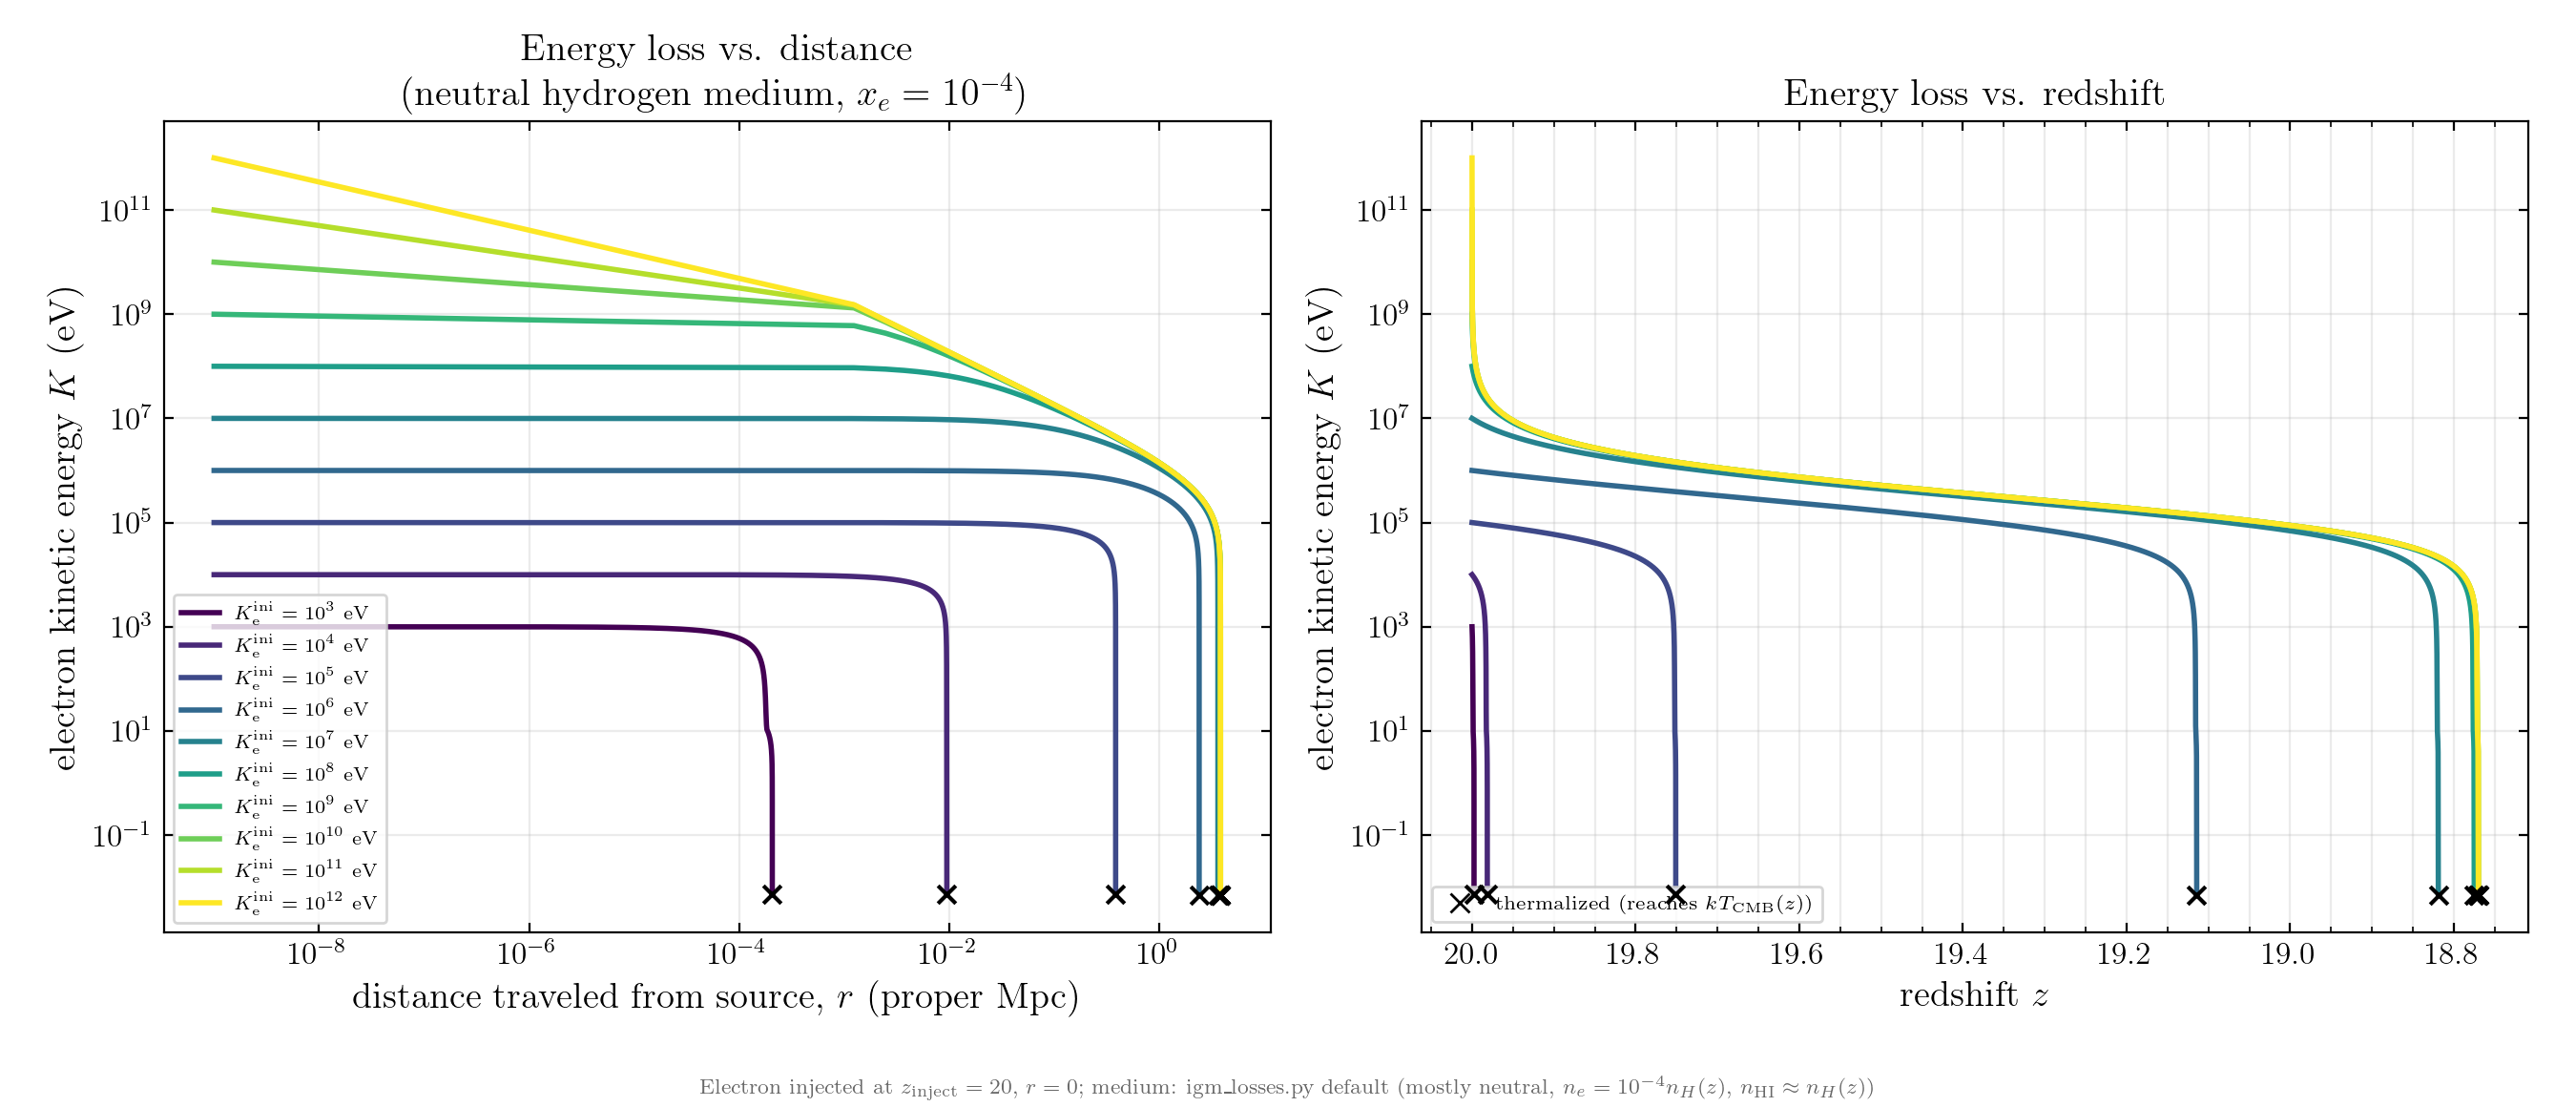
\includegraphics[width=0.92\textwidth]{electron_energy_loss_neutral_medium.png}
\caption{Electron kinetic energy $K$ vs.\ distance traveled (left) and vs.\ redshift (right), for the
neutral hydrogen medium ($x_e=10^{-4}$), for the same ten injection energies as
\texttt{electron\_energy\_loss\_vs\_distance\_redshift.png}. Produced by
\texttt{electron\_energy\_loss\_neutral\_medium.py}.}
\label{fig:neutral}
\end{figure}

\begin{figure}[h]
\centering
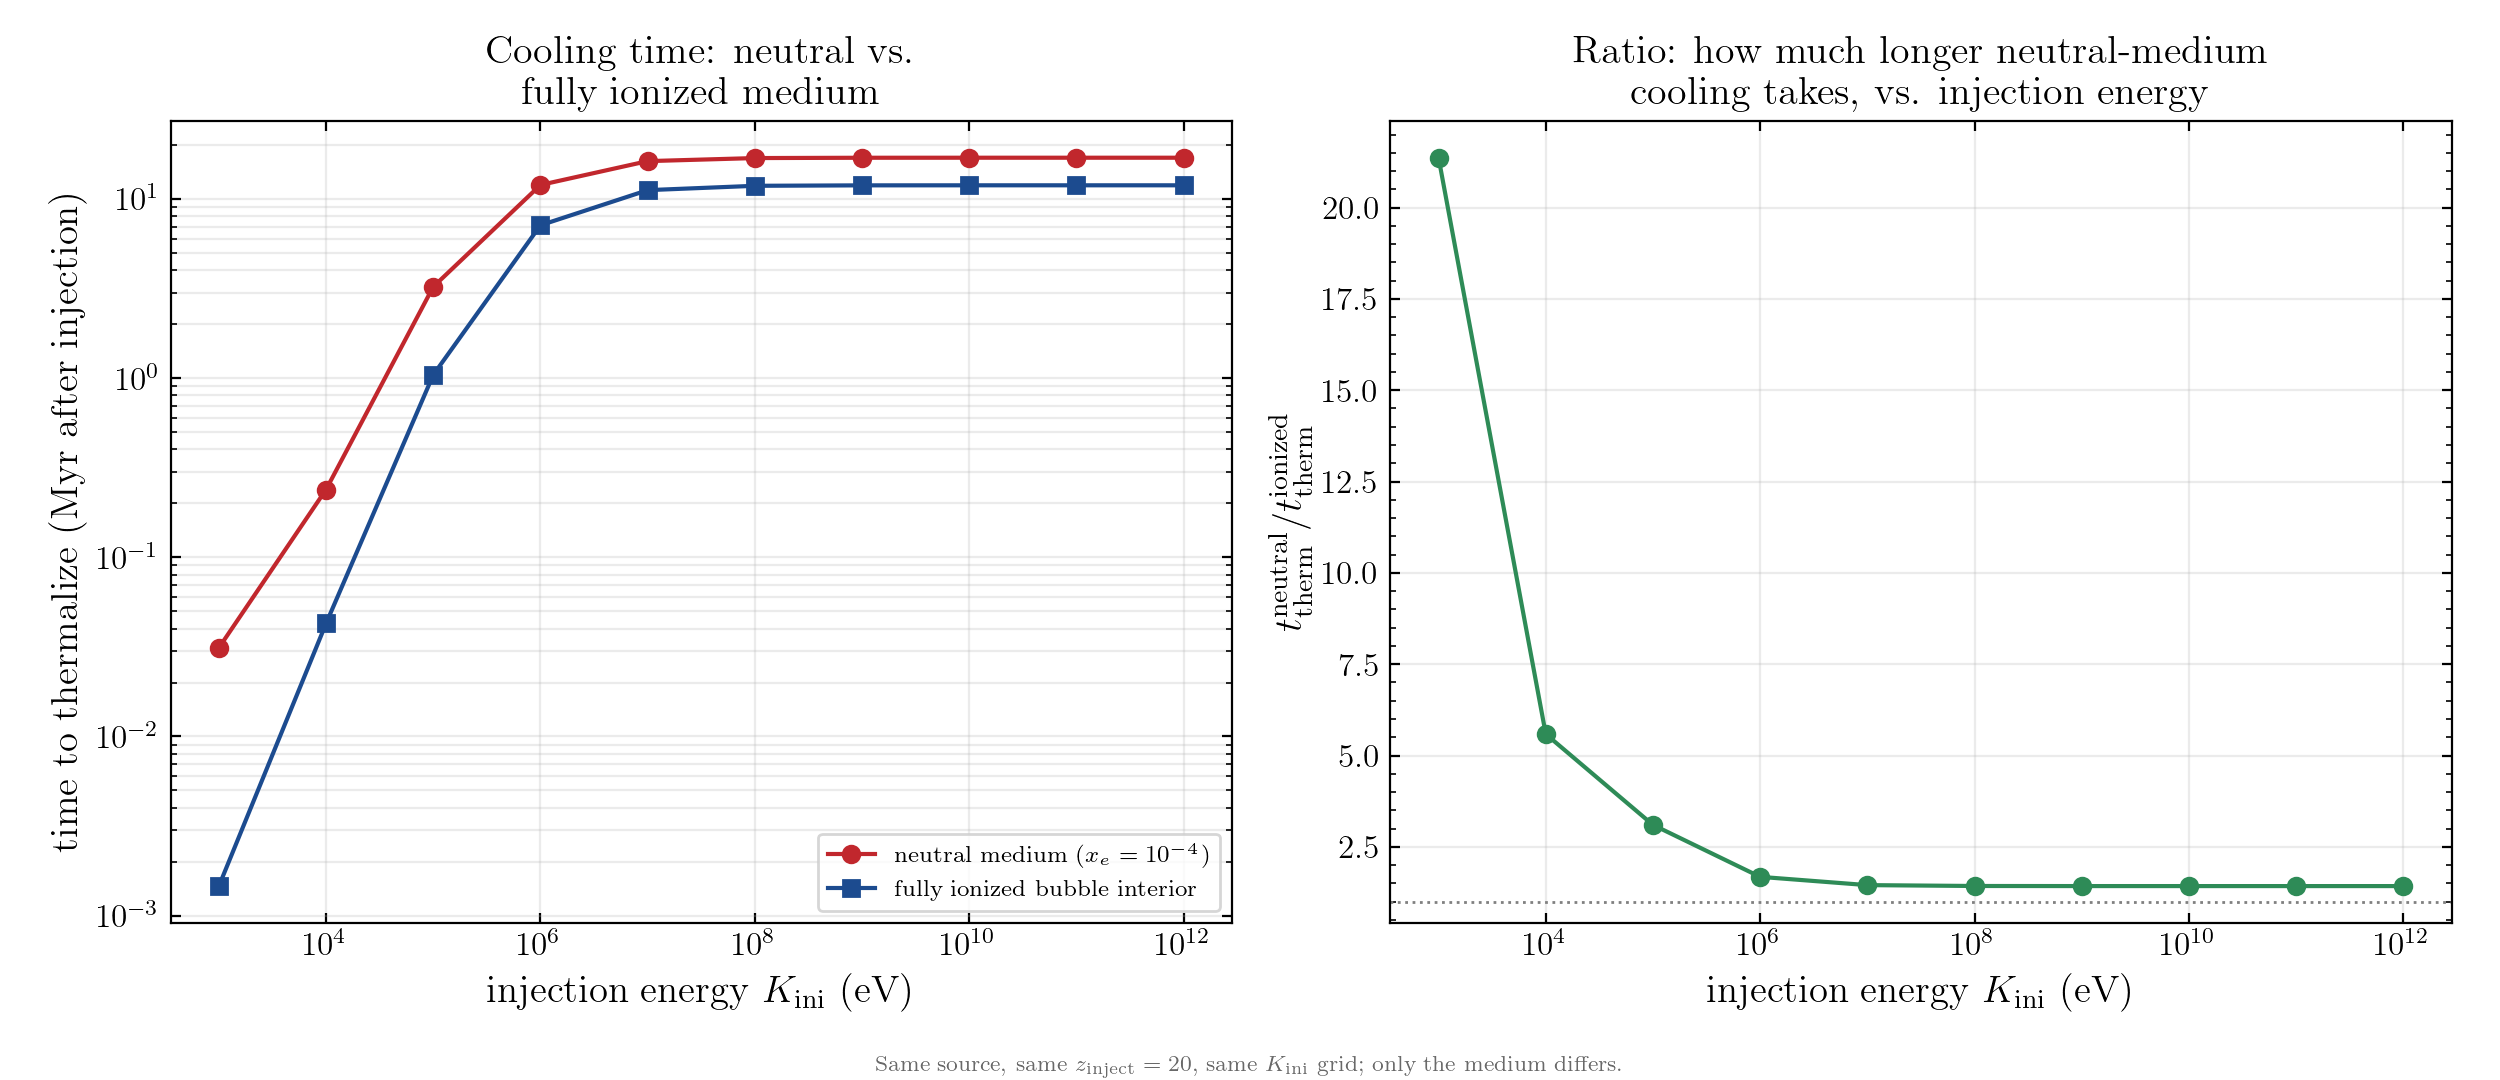
\includegraphics[width=0.92\textwidth]{electron_medium_comparison.png}
\caption{\emph{Left:} time to thermalize vs.\ injection energy, neutral medium (red) vs.\ fully ionized
bubble interior (blue). \emph{Right:} the ratio of the two, showing the $21\times\to1.4\times$ decline
with increasing $K_{\rm ini}$. Produced by \texttt{electron\_energy\_loss\_neutral\_medium.py}.}
\label{fig:comparison}
\end{figure}

%=====================================================================
\bibliography{references}

\end{document}
